\documentclass[10pt,twocolumn]{article} 

% use the oxycomps style file
\usepackage{oxycomps}

% read references.bib for the bibtex data
\bibliography{references}

% include metadata in the generated pdf file
\pdfinfo{
    /Title (The Occidental Computer Science Comprehensive Project: Goals, Format, and Advice)
    /Author (Justin Li)
}

% set the title and author information
\title{The Occidental College Computer Science Comprehensive Project Proposal: \\ Predicting Cryptocurrency Prices for Stock Trading Using Machine Learning}
\author{Odelia Putterman}
\affiliation{Occidental College}
\email{putterman@oxy.edu}

\begin{document}

\maketitle

\begin{abstract}
    This paper is my Occidental College Computer Science Comprehensive Project (COMPs) Proposal for my project: \textit{Predicting Cryptocurrency Prices for Stock Trading Using Machine Learning}. This project proposal has seven components, one for each of: introduction, problem context, technical background, methods, evaluation, ethical considerations, and software documentation.  I begin by introducing the project, then I address the technical aspects of realizing this work, and I end with the ethical concerns regarding this assignment. In tackling each of these sections, I outline the motivation for this work, ethical considerations, and how to produce this project.
\end{abstract}


\section{Introduction}

For my senior-year Occidental College Computer Science Comprehensive Project (COMPs), I have chosen to build an index fund for cryptocurrencies, with rebalancing occuring dynamically in response to crypto price predictions from a machine learning (ML) algorithm. This proposed index fund will utilize the volatility of cryptocurrencies to maximize gains by dynamically trading index fund stocks rather than rebalancing on a preset schedule.

\section{Problem Context}

Investing is a means by which people can grow their money exponentially, but it also holds the potential for significant loss, especially in the context of day trading.

\subsection{Index Funds: Explained}

As it stands, it's difficult, if not impossible, to predict the exact performance of individual stocks. As such, people invest in index funds, collections of stocks which follow some set of rules for construction, to mirror the whole market rather than a particular holding. Such funds are generally mutually pooled, with the stock holdings shared across many holders.

Money that goes into the fund is invested in all the stocks the fund holds, growing the diversification of the fund and minimizing its dependence on individual stock performance. Further, index funds are periodically re-balanced to offset losses and risk, and companies are sold once they leave these predefined rules or parameters discussed.

\subsection{Cryptocurrencies: Unique Opportunity and Approach}

Index funds are generally constructed using fundamental measures of a company (aka fundamentals), such as cash flow, sales, and dividends. Cryptocurrencies, however, have none of these intrinsic metrics. Since the cryptocurrencies themselves are a currency rather than a materialized product, there are no sales or dividends to be found. Their only measure is price. Accordingly, any approach to creating and maintaining a cryptocurrency index fund must be revolutionary in nature.

Cryptocurrencies are incredibly volatile, making re-balancing especially important. Their instability also offers a unique opportunity for leveraging their turning points to optimize gains if high-accuracy price prediction can be achieved. If we could predict cryptocurrency prices in advance, we could leverage this knowledge to maximize gains while keeping a sense of security with the breadth of the fund.

Typically, index funds are rebalanced on a consistent, preset schedule, such as the third Friday at the end of each calendar quarterly. But, what if we could predict cryptocurrency prices to decide how and when to rebalance such a cryptocurrency fund instead? If this succeeded, the results would be revolutionary in nature and a first-of-its-kind for maintaining a balanced, high-return cryptocurrency fund.

People have previously attempted to predict the behavior of cryptocurrencies with some success. I aim to follow in their steps with a slightly different approach and following implementations. Such prior work is discussed below under \textbf{Prior Work}.


\section{Technical Background}

Here I introduce the technical background required to fully comprehend the methods this project undertakes.

\subsection{What Are Cryptocurrencies?}

This comps project involves cryptocurrencies, a relatively new phenomena stemming from advances and uses of blockchain technologies. Cryptocurrencies were first created for their supposed safety and security arising from their basis in blockchain technology. According to \citetitle{WhatIsBlockchain}, ``Blockchain is a shared, immutable ledger that facilitates the process of recording transactions and tracking assets in a business network". Each transaction is recorded as a ``block" of data, connected to the blocks before and after it in an irreversible chain (aka a blockchain).

\subsection{Sentiment Data and Sentiment Analysis}

Sentiment data is essentially the same as it sounds: it is data which signifies sentiment. Sentiment analysis, similarly, is the use of computational algorithms to study subjective information (i.e. sentiment). It is particularly important for understanding the social sentiment of a given thing \cite{SentimentAnalysisConcept}. In the context of this project, the sentiment data is data which can be analyzed to search for crowd feelings on cryptocurrencies, while the sentiment analysis is the analysis of this data to learn attitudes towards cryptocurrencies.

\subsection{What are LSTMs?}

Long-short term neural networks (LSTMs) are a type of neural network or, more specifically, recurrent neural network (RNN). To explain what LSTM neural networks are, we must first explain what RNNs are.

\subsubsection{RNNs}

We begin by introducing RNNs. RNNs are a type of neural network capable of learning order dependence, which is key in sequence prediction problems. They differ from traditional feedforward neural networks, or multilayer perceptrons (MLPs), in their inclusion of feedback connections. Feedback connections are when outputs of a model are fed back into itself \cite{DeepLearningFeedforward}. To be an RNN, a system must

\begin{enumerate}
    \item be able to store information for an arbitrary period;
    \item be resistant to noise (i.e. random inputs, outliers, etc.); and
    \item have trainable system parameters.
\end{enumerate}

In RNNs, the \emph{context} is learned, meaning an RNN contains cycles which feed the network outputs, or activations, from a prior time step as input to the network for future time steps. However, they fail to ``remember" things from far back. RNNs are susceptible to backpropagated error. RNNs have hidden layers which can decay or blow up when circling around a feedback connection \cite{GentleIntroductionToLSTMNetworks}. Essentially, layers in RNNs with small enough gradient updates stop learning, usually in relatively early-on layers, causing short-term memory, or what is known as the vanishing gradient problem, while layers with large enough gradients exponentially grow towards infinity, causing a blow-up problem and an unrealistic expectation for reliance on unimportant, or not as important as is implied, information \cite{IllustratedGuideToLSTMs}. RNNs typically perform poorly on time-series sequential problems, as this backpropogated error will either cause exponential blowing up or the vanishing gradient problem, the decay of important learned information \cite{GentleIntroductionToLSTMNetworks}. This poses a major challenge to accurately making predictions for sequential operations with a stratified breakdown. This leads us to an important variation on traditional RNNs, and the topic of this paper: LSTMs.

\subsubsection{LSTMs}

LSTMs are a subset of recurrent neural networks (RNNs), similar in most respects, introduced in 1997 by Hochreiter and Shmidhuber \cite{UnderstandingLSTMs}. LSTMs differ from RNNs in their ability to solve the vanishing gradients and exploding gradients problems. Like RNNs, they learn order dependence in sequence prediction problems, only they are far more effective at retaining both long-term and short-term memory. They can keep information about the past for a unfixed period, to be decided by the input data weights as feedback connections are formed throughout the neural network operations; they use contextual information flexibly. LSTMs can traverse longer time steps to store important information with a constant error flow, avoiding the RNN problem or exponential blowing-up and decay \cite{GentleIntroductionToLSTMNetworks}. These feedback connections, or loops, allow for the persistence of information in traditional RNNs, and, correspondingly, LSTMs. RNNs, and, accordingly, LSTMs, can be thought of as multiple copies of the same network, each passing information to the succeeding network. When the gap in knowledge from the prior input information to the next is relatively small, an RNN may succeed. But substantial research shows LSTMs far outperform typical RNNs when more context is needed \cite{UnderstandingLSTMs}. As an example, let us look at the sentence:

\begin{quote}
    I have been following the Tesla stock price performance for months... I am going to invest in \emph{Tesla}
\end{quote}

The segment ``invest in" suggests the following word will be a company, stock, or object. To come to the conclusion that this person will invest in Tesla, we need the earlier context that this person has been following the Tesla stock price. In this analogy, an RNN would have the memory to know the following word will be a company, stock, or object, but it would have lost the context of Tesla, rendering it unable to correctly predict the following word, unlike an LSTM which, having successfully kept this context, would be better fit to make an educated decision.

\subsubsection{How LSTMs Work}

The principal idea which separates LSTMs from traditional RNNs is the \emph{cell state} and its corresponding \emph{gates} \cite{UnderstandingLSTMs}. The cell state is what runs along these `copies' of the network, changing its state as it covers the chain of networks (network over time steps), removing and/or adding information to its state with these gates as it goes \cite{IllustratedGuideToLSTMs}. In this way, the cell state can be thought of as the network's memory; it is the compilation of `relevant' information, or memory cells, at any given point in time; it is a series of recurrently connected memory blocks. LSTM neural networks are comprised of one or more recurrently connected memory cells with their respective gates \cite{GentleIntroductionToLSTMNetworks}. Gates are basically different neural networks which decide which information should be in a cell state; they learn what constitutes `relevant' information during their individual training(s) \cite{IllustratedGuideToLSTMs}. There is a constant error flow within the constant error carousel (CEC), and these gates learn to control access to this error flow within each memory cell's CEC \cite{GentleIntroductionToLSTMNetworks}.

LSTMs have three layers or inputs: an input layer, a hidden layer, and an output layer. The input layer is the input data given to the network at that given time step; the hidden layer is the compilation of memory cells and corresponding gate units; and the output layer is the output information to be passed to the following time step, to complete the feedback connection unique to RNNs \cite{IllustratedGuideToLSTMs}.

LSTMs have three to four gates, depending on how you look at their breakdown. These are either a forget gate, an input gate, and an output gate \cite{GentleIntroductionToLSTMNetworks} or a forget gate, a learn gate (aka input gate), a remember gate (aka candidate gate), and an output gate \cite{HowLSTMsWork}. For the purpose of this paper, we will explain LSTMs using the four gates formulation.

\begin{figure}
    \centering
    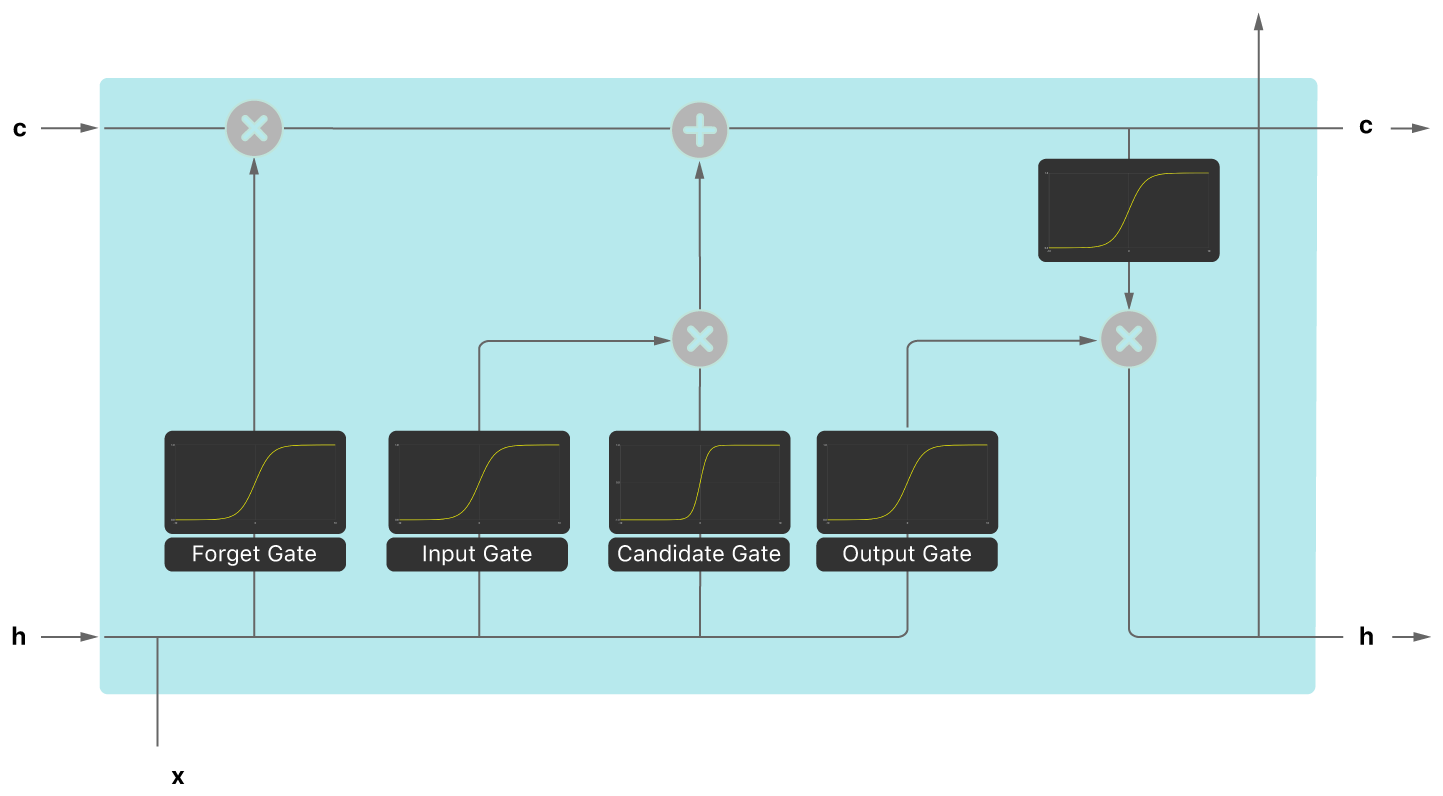
\includegraphics[scale=0.15]{images/four_layers.png}
    \caption{
        Sketch of the four gates and their connections from \cite{LSTMMemoryLayers}.
    }
\end{figure}

Note, the long-term memory (LTM or `$C$') is the cell state, the short-term memory (STM or `$h$') is the hidden layer, and the input data (`E' or `$x$') is the newly given information at this time-step.

\paragraph{Forget Gate}

The forget gate, a sigmoid layer, decides what information should be thrown away or kept. The input parameters to this gate are the previous hidden state (hidden state from `preceding' network), aka the output from the preceding neural network or short-term memory/information ($h_{t-1}$), and the current neural network input $x_t$ \cite{UnderstandingLSTMs} or just the cell state \cite{HowLSTMsWork} if taking the four-step gate approach, as we have decided to do.

The forget gate output values between 0 and 1 using a sigmoid activation (function) for each value in the passed in cell state $C_{t-1}$ \cite{UnderstandingLSTMs}. A sigmoid function will simply compress the given value to a value between 0 and 1. This is helpful in forgetting and remembering information, as values multiplied by 0 disappear (are `forgotten') and values multiplied by 1 will stay the same (are `remembered'). This forget gate tells the network at that time step which information is important to keep and what information it can forget \cite{IllustratedGuideToLSTMs}.

This gate multiplies the state long-term information by a forget factor $f$ to `forget' some of this long-term information.

\[
f_t = \sigma(W_f[h_{t-1}, x_t] + b_f)
\]

This forget factor $f$ is what gets multiplied against the values in the  state's long-term information to decide what to keep and what to forget \cite{HowLSTMsWork}.

\paragraph{Learn Gate}

The learn gate's input parameters are the hidden layer ($h$), or short-term memory, from the previous time-step and the current network input `x' \cite{HowLSTMsWork}. The learn gate protects the CEC from altering due to unimportant inputs using useful multiplication \cite{GentleIntroductionToLSTMNetworks}. This gate uses a tanh layer to create a vector of new $\tilde{C}_t$ values which can be added to the cell state \cite{UnderstandingLSTMs}.

\[
\tilde{C_t} = tanh(W_c[h_{t-1}, x_t] + b_c)
\]

We need to ignore some of the short-term memory, which we achieve by multiplying the combined result by an ignore factor $i$, calculated by combining the short-term memory and new information with a new set of weights and biases.

\[
i_t = \sigma(W_i[h_{t-1}, x_t] + b_i)
\]

Once $\tilde{C}$ and $i$ are calculated, they are multiplied together. This multiplication yields the learn gate output, to be passed to the remember gate. This learn gate, in essence, learned the new input information `x' \cite{HowLSTMsWork}.


\paragraph{Remember Gate}

This gate computes the new long-term memory by adding the the output of the forget gate with the output of the learn gate.

\[
C_t = learn + forget
\]

\[
C_t = f_t * C_{t-1} + i_t * \tilde{C_t}
\]

\paragraph{Output Gate}

The output gate decides what the next hidden gate (to be passed to the succeeding network) should be. The output gate protects changing other units (succeeding time steps) from changing due to current irrelevant memory \cite{GentleIntroductionToLSTMNetworks}. It passes the newly modified cell state to a tanh function, which will compress all its input values to values between -1 and 1, and multiplies the output of this tanh activation with the sigmoid activation output to decide which information the hidden state should hold. The output of the output gate, as mentioned, is this newly corrected hidden state \cite{IllustratedGuideToLSTMs}.

This gate takes the outputs from the forget and learn gates to create a new hidden layer (aka short-term memory). It takes the output of the learn gate and applies a sigmoid function on it.

\[
O_t = \sigma(W_{\sigma}[h_{t-1}, x_t] + b_{\sigma})
\]

Finally, it multiplies $O_t \times tanh(C_t)$ to get the new hidden layer, or short-term memory \cite{UsingLSTMInStockPricePrediction}.

\[
h_t = O_t \dot tanh(C_t)
\]

The new hidden state and cell state are carried to the next time step, and this whole three-layer process is repeated \cite{IllustratedGuideToLSTMs}.


\subsection{Index Fund Rebalancing}

Index fund rebalancing is the process of rebalancing is the process of selling and buying stocks to balance the distribution across a fund.

There are many ways to rebalance an index fund. The usual choice is \textbf{calendar rebalancing}. In calendar rebalancing, the index fund holdings are reviewed on a preset calendar basis and adjusted to their original form. The actual rebalancing is done by examining issues such as transaction costs and drifts.

Another type of rebalancing, later discussed, is \textbf{percentage-of-portfolio rebalancing}. According to \citetitle{TypesOfRebalancingStrategies}, percentage-of-portfolio rebalancing is a ``rebalancing schedule focused on the allowable percentage composition of an asset in a portfolio. Every asset class, or individual security, is given a target weight and a corresponding tolerance range."

There are many other types of rebalancing algorithms, but these are the two most important rebalancing algorithms to understand for the scope of this project.

\subsubsection{Calendar Rebalancing}

\subsubsection{Percentage-of-portfolio Rebalancing}

\section{Methods}

I propose to predict cryptocurrency prices using machine learning, specifically an LSTM neural network, and sentiment analysis. Because, as previously mentioned, cryptocurrencies don’t have fundamentals, we must evaluate and try to predict their behavior using other metrics for input data. Here, I propose the use of sentiment analysis.

\subsection{Language of Choice}

My language of choice for this project is Python using Google Colab. Python is my language of choice for its abundant scraping and machine learning libraries/tools in addition to its simplicity of use. Accordingly, all libraries discussed are Python libraries. Google Colab will also be used for its access to GPUs for network training purposes.

\subsection{Sentiment Analysis Input Data}

Originally I thought to use both sentiment analysis and current events data for cryptocurrency price prediction. But, after realizing the complexity involved in this project, I chose to stick with just sentiment data since, ideally, sentiment should mirror current events; any major disarray which may affect crypto prices will likely be expressed in sentiment towards the currency.

Such sentiment, in this case, should convey feelings towards or about cryptocurrencies. This sentiment can be sourced form news articles, social media posts, and other messaging. Input data for sentiment analysis should include, but is not limited to:

\begin{itemize}
    \item The number of positive and/or negative news articles about specific cryptocurrencies/cryptocurrency (as a concept) generally;
    \item The number of positive and/or negative social media posts about specific cryptocurrencies/cryptocurrency (as a concept) generally; and
    \item The number of positive and/or negative crypto blog postings about specific cryptocurrencies/cryptocurrency (as a concept) generally.
\end{itemize}

As I continue my project research, I plan to add more input sources on which to perform sentiment analysis to gather crowd feelings towards cryptocurrencies.

\subsection{Obtaining Data for Sentiment Analysis}

Now that we have determined which data to analyze, we must consider how this data will be acquired. Ideally, there would be preset datasets with this information. But, I have yet to find any with the breadth, depth, and upkeep necessary for such a machine learning algorithm to succeed. So, unless I find an ideal dataset, scraping is my preferred method for training and maintenance data acquisition. I don’t want my project to be about how to scrape data, rather I’d like to make this as painless as possible. To prevent scraping itself becoming a massive project, I plan to use existing libraries for help tackling this problem, such as:

\begin{itemize}
    \item PyGoogleNews;
    \item NewsCatcher;
    \item FeedParser; or
    \item NewsPaper3k.
\end{itemize}

Cryptocurrencies are a global phenomenon, so we should not limit our scope of search to US-based sites. But, this is still a college project with limitations to its scope, so I plan to start with sourcing articles written in English from mostly US-based cites, but eventually (if time permits) broaden my scraping to more non-US websites and, potentially, other languages.

I plan to narrow my list of sentiment data sources and scrape from these to get the training data and periodically retrieve classification data for price prediction. Below, I list sources I suggest be scraped for input data to the sentiment analysis.

\subsubsection{News Sources}
\label{sec:newssources}

\begin{enumerate}
    \item The New York Times
    \item The Economist
    \item CNN
\end{enumerate}

\subsubsection{Social Media}

\begin{enumerate}
    \item Instagram
    \item Facebook
    \item Twitter
\end{enumerate}

\subsubsection{Crypto Blogs}

\begin{enumerate}
    \item Cointelegraph
    \item NewsBTC
    \item CryptoNinjas
\end{enumerate}

Most of these should be available to be openly viewed or have APIs which could be connected for scraping. This scraping would look for occurrences of each of the aforementioned datapoints and add them to an input array, potentially spanning the course of a few hours to a week (time range to be decided), to be fed into a sentiment analysis algorithm.

\subsection{Sentiment Analysis to LSTM Input Data}

To decipher this sentiment, I will use an existing natural language processing (NLP) algorithm. Possible libraries for sentiment extraction are:

\begin{enumerate}
    \item NLTK (Natural Language Toolkit);
    \item SpaCy;
    \item TextBlob;
    \item Stanford CoreNLP; and
    \item Gensim.
\end{enumerate}

This sentiment analysis will result in a csv files that list the date, source, and sentiment analysis result for each sentiment datapoint for each cryptocurrency, which will then be passed forward to the LSTM neural network for cryptocurrency price prediction and training.

\subsection{Predict Cryptocurrency Prices with LSTM Neural Network}

Deep learning models are novel in their classification capabilities, and with decreasing compute times, they are an increasingly affordable option. But traditional deep learning models are not able to store contextual information, lacking the persistence necessary for sequential predictions, such as stock price predictions. The need for a method capable of time-sensitive sequential predictions leads us to recurrent neural networks (RNNs), or, more fittingly, long-short term memory (LSTM) neural networks.

LSTMs are a great candidate for time-series predictions such as stock price predictions. Since they are able to use historical information and continuously contextually decide what information is relevant, they are able to more effectively return on such sequential problems. To solve the stock price prediction problem.

For all these reasons, to predict cryptocurrency prices, I suggest the use of LSTM neural networks. Possible libraries for building and training an LSTM neural network to perform this task are:

\begin{itemize}
    \item TensorFlow;
    \item PyTorch;
    \item NeuroLab; and
    \item Scikit-Neural Network.
\end{itemize}

The LSTM will be inputted the output from the sentiment analysis step and output a csv file with future dates and corresponding cryptocurrency price predictions by cryptocurrency, to be inputted to the rebalancing trading algorithm.

\subsection{Feed ML Outputs to Trading Algorithm}

A key idea to the success of this project's proposed index fund is the use of cryptocurrency price predictions to rebalance a proposed index fund dynamically rather than on a preset schedule. My choice of rebalancing is a mixture between calendar rebalancing and percentage-of-portfolio rebalancing, where basically every given period of time (ideally deciphered by an ML algorithm as when prices are dramatically changing), I would rebalance the portfolio to mitigate risk but maximize profits with percentage-of-portfolio rebalancing. This will result in the proposed cryptocurrency index fund.

\section{Evaluation}

To evaluate the success of these models, I plan to feed the model data from after the training period and compare the outputted cryptocurrency price prediction results against the actual cryptocurrency prices from that time to see if the LSTM neural network succeeded.

To evaluate the success of the cryptocurrency index fund itself, I will compare the year-to-date (YTD) success of the sentiment analysis based LSTM neural network and index fund trading algorithm - potentially multiple funds based on different NLP algorithms, ML algorithms, and training datasets - with the YTD success of common cryptocurrency index funds (i.e. ProShares Bitcoin Strategy ETF, Grayscale Bitcoin Trust, Bitwise 10 Crypto Index Fund...).

Based on how each model performed, we can answer some follow up questions to maximize the accuracy of the cryptocurrency price prediction algorithms and index fund:

\begin{itemize}
    \item How did the price-prediction-based trading algorithm perform?
    \item Should we use one or another cryptocurrency price prediction solely to inform the cryptocurrency index fund trading algorithm?
\end{itemize}

\section{Ethical Considerations}

When considering the ethical considerations of predicting cryptocurrency prices for stock trading using machine learning, we must break the question into sub-tasks. Since this project advocates for the use of cryptocurrencies, we must consider the ethics of cryptocurrencies themselves. Further, we must look into the ethics of stock trading and the investor obligations that come into play when building an index fund, especially one built with machine learning.

\subsection{Nature of Cryptocurrency}

Due to the immutability of blockchain, and, hence, cryptocurrencies, the risk of tampering by bad actors is eliminated, creating a trustworthy network. Traditionally, information storage and retrieval systems were susceptible to cyberattacks. Moreover, without transparency on behalf of the record-management company or system, record tampering would be harder to catch and verify. The open-book nature of blockchain allows for widespread verification of all transactions. Coupled with the blockchain's immutable nature, with no user nor managing power having the ability to alter or delete a transaction, blockchain technologies, and, hence, cryptocurrencies, are extremely safe from a tampering standpoint \cite{WhatIsBlockchain}. This addresses transparency on behalf of the cryptocurrency operations, but it does not cover the ethical considerations with regard to the security of such assets.

A second consideration is the instability of where cryptocurrencies are hosted. One Washington Post Article, \citetitle{TrackingStolenCrypto}, details the commonality of crypto heists. Hackers have previously hacked into cryptocurrency trading networks, getting away with massive sums. In August of 2021, Poly Network, a trading platform for popular cryptocurrencies, was hacked, with the hackers taking 
\$610 million in crypto, which they quickly converted to a ``stable coin". Luckily, the ``stable coin" Tether worked with authorities to release the holdings to the rightful owners. Nonetheless, this heist broke the belief that cryptocurrency is impossible to trace (public ledgers do not retain account holder information) \cite{TrackingStolenCrypto}. The anonymity of cryptocurrencies may be ethical, guarding the identity of its users or not, allowing for bad actors to use crypto for illicit activities, but it is certain that their online holdings make them susceptible to being stolen, further questioning the security of their nature.

Despite the secure theoretical ideas behind cryptocurrencies, their value is often in flux. Ethicists have previously questioned the ethics of cryptocurrencies themselves. Professor Tobey Karen Scharding shared her evaluation of bitcoin from an ethical perspective in an interview at Rutgers Business School:

\begin{quote}
    My question was, is Bitcoin an ethical currency not is it ethical to use bitcoin or is it ethical to trade some dollars for bitcoin... With bitcoin, I felt there were too many uncertainties... [The] evaluation was pretty negative because bitcoin didn't really have any way to secure its value, and so it wouldn't be able to fulfill the ethical purpose of currency on Fichte's account of stabilizing and securing these exchanges over generations. \cite{IsBitcoinEthical}
\end{quote}

Professor Scharding refers here to the Fichte account, which explains that currency should allow people to live their lives with secure access to basic goods and services and allows them to enjoy life and exchange goods with other people. By Professor Scharding's logic, cryptocurrency falls short of being an ethical currency because its often-changing value means that one day it could secure these assets and more for a given holder while the next day it could be deemed worthless, leaving the holder unable to meet these basic needs. That said, she believes cryptocurrencies could become ethical if an entire nation takes on cryptocurrency and stabilizes its value \cite{IsBitcoinEthical}.

\subsection{Investor Obligations}

Managing an index fund holds a moral obligation to the holders to aim to grow their investment. Cryptocurrency price prediction carries inherit risk. A major concern is the volatility of cryptocurrencies. Though we seek to leverage this volatility, it could also be a major pitfall if prices are incorrectly predicted. In this proposed fund, if the crypto prices are wrongly predicted, funds will likely get misallocated and, in turn, lose the investor money. If the machine learning algorithm wrongly predicts the coming crypto prices, we risk losing investor money and being an unethical project, as it promotes investing with no return. To uphold our ethical obligation to investors, we must strive for the highest level of accuracy in this work.

\subsubsection{Data Bias}

Data Bias is a massive consideration to take into account when analyzing the results of machine learning projects. All machine learning, regardless of the task, shares a reliance on input data for learning and training. And, according to \citetitle{RiskOfMachineLearningBias}, ``[The] models learn exactly what they are taught". This input data heavily affects the model's outcome. As data scientists classically say, ``garbage in, garbage out". In training the model for this comps project, in order to not receive ``garbage out" and lose investor money, we must ensure the input data is not biased. Since this machine learning project takes in sentiment data and outputs a price prediction for each cryptocurrency, there is no fear of outputting politically incorrect and dangerous results. But, there is a fear that biased input data will lead to biased price predictions, which would, in turn, lose investor holdings. Such bias could result from only looking at certain web sources which portray a biased sentiment towards cryptocurrencies or from not properly analyzing the given sentiment. To avoid wrongly predicting crypto prices and failing the fund investors, we must ensure high-quality data is being fed into the algorithm.

\subsubsection{Model}

Cryptocurrency prices are extremely volatile, making their price prediction a uniquely difficult challenge. The likelihood that this comps project were to succeed in accurately predicting cryptocurrency prices consistently is incredibly low. This leaves a high likelihood  of inaccurate predictions at some point, if not frequently, which has greater implications on the ethical consideration of investor obligations, model transparency, and security. Promoting the practice of placing a monetary commodity in cryptocurrencies is ethically dubious, as it holds high risks of loosing this money, threatening the financial security of such investors.

To make this project more ethical, there is a need for a lot of transparency on the risks involved in investing in this comps project intended fund due to the accuracy rates of the developed machine learning model and the extremely volatile nature of the assets involved.

\subsection{Investing}

To explore the ethics of this investing-based project, we ask, \textit{is investing itself fair?} In investing, we subscribe to a system where the wealthy have an infinitely easier time to build more wealth than the poor do. The stock market is an inherently unfair playing field. Due to the compound nature of investing and investments, it is infinitely easier to become wealthy if you are already wealthy than it is to turn a little into a lot; the stock market favors those who start off with more. By this logic, it appears to be an unethical system.

We can, however, approach ethical investing from another standpoint. Rather than concern ourselves with the ethics of investing itself, we can ask how to ethically invest money. There is a growing field of learning around \textit{ethical investing}. Ethical investing has many different approaches, but the idea is to use investing as a tool to do good. Manisha Thakor, a financial planner and consultant, says, according to \citetitle{LimitsOfEthicalInvesting}, ``The broad idea behind this style of investing is a belief that you can generate meaningful, measurable, societal outcomes while also generating a healthy profit". You can put your money towards companies addressing an ethical issue, such as climate change, racism, or workplace inequality while also generating wealth. The three overarching areas for ethical investments are environment issues, societal issues, and governance issues \cite{LimitsOfEthicalInvesting}. Cryptocurrencies do not fall under environment issues to the best of my knowledge, but they can, arguably, fall under societal and governance issues.

For starters, cryptos can help in enabling financial inclusion. As \citetitle{CryptocurrenciesFinancialInclusion} says, ``The crypto economy is leading to the development of an alternative financial and technological infrastructure that is global, open source, and accessible to all who have access to the internet, regardless of nationality, ethnicity, race, gender, and socioeconomic class... not enough of us are rolling up our sleeves and getting involved with building this new global and inclusive open financial system". By this framework, cryptocurrencies have the power to do extreme good, and investing in them allows us to "[roll] up our sleeves and [get] involved with building this new global and inclusive open financial system", allowing for greater financial inclusion and opportunity worldwide, a pivotal societal and governance problem.


\subsection{Accessibility}

Another ethical concern this project faces is accessibility. We must consider:

\begin{itemize}
    \item Is it fair that only some have access to crypto price predictions?
    \item Is it ethically right to make such crypto price predictions widely available?
    \item If crypto price predictions are made widely available, will the prediction itself alter the crypto prices, creating self-fulfilling, `announcement-driven' outcomes?
\end{itemize}

We navigate each of these questions in the below sections.

\subsubsection{Power Distribution}

As it stands, ``the rich get richer". If this comps project achieved any level of success in predicting cryptocurrency prices, there would be a question of \textit{who} gets access to these predictions. If these predictions were offered as a subscription service with a high buy-in, the buyers would most likely be those wealthier individuals, giving the elite investors a tool not readily available to the average investor, making it continuously easier for the wealthy to keep get wealthier while the poor get poorer. If these predictions or this fund were expensive and exclusive, we risk contributing to the wealth divide and creating further disparity in power distribution. If instead we choose to make this tool openly accessed, we run into other ethical problems.

\subsection{Self-Fulfillment}

Imagine now that everyone had access to this crypto price prediction tool and that it operated with some meaningful level of accuracy. If these predictions were so easily accessed, it is entirely possible that the predictions would become self-fulfilling cycle where:

\begin{enumerate}
    \item Price predictions are publicized;
    \item People buy stock when its predicted to be rising in price and sell it when it is predicted to fall in the coming future;
    \item These prediction-based purchases drive up or down the crypto.
\end{enumerate}

If this were to happen, no \textit{actual} predicting would be helpful, and all people would not be benefited by such predictions. As such, it is important that the price prediction component of this comps project be kept private, with only the fund performance made available.

\subsection{Maintenance and its Environmental Cost}

Maintaining the proposed index fund requires constantly retrieving sentiment data, performing natural language processing (a type of ML) on this data, feeding the outputs of the NLP sentiment analysis data to an ML algorithm for price-predictions, and feeding the ML outputs to a rebalancing algorithm for the index fund. These operations have an environmental impact and cost in addition to the initial cost of training these individual models. This comps project will utilize a recurrent neural network (RNN), a type of deep learning model. In a 2019 study at the University of Massachusetts at Amherst, it was approximated 626,000 pounds of carbon dioxide are used in training a large deep-learning model \cite{ShrinkingDLCarbonFootprint}. Though, in practice, this comps project will not consist of a large deep-learning model, in theory, this project should be executed with the use of a large model to boost accuracy in price predictions. The environmental impact of training and up-keeping such an RNN should not be taken lightly. Training and continuously processing information for this price-prediction project takes a tremendous amount of energy, which has a real-world environment cost.

The second consideration is the environmental impact of cryptocurrencies, as they are the `product' being promoted by this project. Bitcoins enter circulation through \textit{mining}, a process of validating new blockchain transactions. When a transaction is requested to be processed, \textit{miners} race to be the first to get their validation accepted by solving a challenge, where their validation validates and record a bundle of new transactions, bundled into a \textit{block}, as the first miner to complete this process is awarded with new bitcoin and transaction fees. As crypto prices surge, more miners enter the race to win some crypto. Moreover, as more miners enter the race, the processing protocol makes it more difficult to win this race, by finding the \textit{nonce}, whereas when there are fewer users, the system makes this validation process and puzzle easier, all in the effort to keep block production time to ten minutes. It is approximated that there are around one million bitcoin miners. A lot of energy is spent from all these users aiming to mine bitcoin with their computing power. The University of Cambridge estimated bitcoin mining uses 121.36 terawatt hours a year \cite{BitcoinImpactOnClimate}. All this makes cryptocurrencies an unfriendly choice for ethicists and environmentalists.

All this said, this project, in actuality, will not consist of large deep-learning model. Rather, it will be the scope of a senior thesis project, resulting in a relatively small neural network. Thus, these environmental concerns do not directly apply, and we are safe to resume this project within the realms of environmental ethical concern.



\section{Software Documentation}


\printbibliography 

\end{document}